\section{Optuna - Hyperparameter Optimization Library}

As defined in the challenges section, hyperparameter tuning is one of the most challenging part of Reinforcement Learning. There are some unique guidelines like with higher batch-size, one can afford higher learning-size. But in general, there is no theoretical foundation that describes hyperparameter selection. In recent years many hyperparameter optimization libraries have been developed to address the issue of parameter selection. Some software designed a tree-structured Parzen estimator like Hyperopt, and some use Gaussian processes like Spearmint and GpyOpt to optimize for the best performing parameters \cite{optuna_2019}. 
Optuna outperforms other optimization software with the following points:

\begin{itemize}
    \item Define-By-Run API 
    \item Better Pruning Strategy
    \item Easy to Setup
\end{itemize}

Define-By-Run interface first coined in the machine learning context. PyTorch surpassed Tensorflow with the help of its dynamic define-by-run API. While in the machine learning framework, Define-By-Run refers to defining the neural network on the go, in hyperparameter optimization, it relates to allowing the user to specify the objective function \cite{optuna_2019}. Optuna takes care of the dynamic construction of the search space. In other words, the user does not need to enter the search space statically.

Interface design only defines how users can interact with the software but give no hint about the performance of the underlying algorithm. For a robust hyperparameter optimization framework, a cost-effective pruning system is a must. Optuna adopts a variant of the Asynchronous Successive Halving algorithm to trigger a background call to the 'should-prune' method \cite{Li2018}.

Optuna is an open-source MIT licensed software. Hence, it attracts a variety of users in the ML world to verify the scalability and robustness. Indeed, it proves to be easy-to-use with over 2.8k stars on their Github page\footnote{\url{github.com/optuna/optuna}}. Moreover, we were satisfied with their documentation and thorough tutorials \footnote{\url{optuna.readthedocs.io/en/stable/}}.

Overall, we were satisfied with the performance of Optuna. Although we didn’t try the other optimization framework, the figure in \ref{fig:hyperparameteropt} represents the high-level comparison to Optuna.

\begin{figure}[htbp]
    \centering
      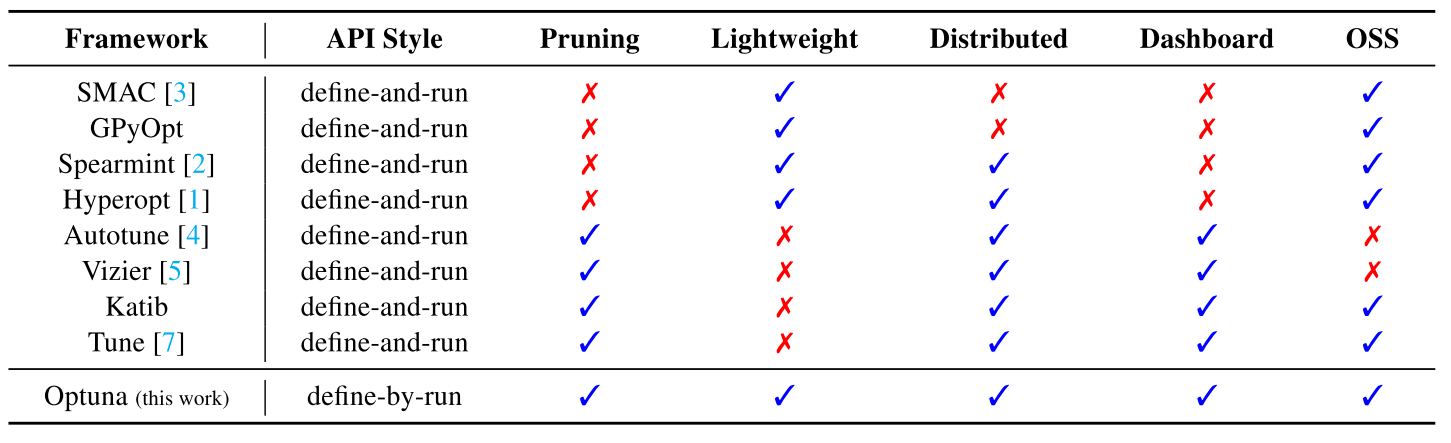
\includegraphics[width=0.9\textwidth]{figures/HyperParam}
    \caption{Hyperparameter optimization library comparison \cite{optuna_2019}}
    \label{fig:hyperparameteropt}
\end{figure}